%----------------------------------------------------------
% Main format settings
%----------------------------------------------------------
\documentclass{beamer}
\usepackage{graphicx}
%\usepackage{authblk}

%\setlength{\textwidth}{16cm}
%\setlength{\oddsidemargin}{0pt}
%\setlength{\evensidemargin}{0pt}
%\setlength{\topmargin}{0cm}
\usepackage{caption} 
%\captionsetup[table]{skip=10pt}
\usepackage{mathtools}
\usepackage{graphicx}
%\usepackage{hyperref}
\usepackage[utf8]{inputenc}
 
\usepackage{listings}
\usepackage{float}
\usepackage{xcolor}
\usepackage{subfig}
\usepackage{mathptmx}
\usepackage[11pt]{moresize}
\definecolor{codegreen}{rgb}{0,0.6,0}
\definecolor{codegray}{rgb}{0.5,0.5,0.5}
\definecolor{codepurple}{rgb}{0.58,0,0.82}
\definecolor{backcolour}{rgb}{0.95,0.95,0.95}
 
\lstdefinestyle{mystyle}{
    backgroundcolor=\color{backcolour},   
    commentstyle=\color{codegreen},
    keywordstyle=\color{magenta},
    numberstyle=\tiny\color{codegray},
    stringstyle=\color{codepurple},
    basicstyle=\ttfamily\footnotesize,
    breakatwhitespace=false,         
    breaklines=true,                 
    captionpos=b,                    
    keepspaces=true,                 
    numbers=left,                    
    numbersep=5pt,                  
    showspaces=false,                
    showstringspaces=false,
    showtabs=false,                  
    tabsize=2
}
\lstset{style=mystyle}
\usetheme{Warsaw}
%----------------------------------------------------------
% Start of the document
%----------------------------------------------------------
\begin{document}

%----------------------------------------------------------
% Title and authors sections
%----------------------------------------------------------
\title{Dirichlet-type Boundary Value Problem}
\subtitle{Using the shooting method and Newton's algorithm}


\author{B. Roque, J. Jiménez, J. Caraballo, P. Negr\'{o}n}
\institute{Department of Mathematics, UPR-Humacao}
\date{\today}

%%%%%%%%%%%%%%%%---- AQUI EMPIEZA -----%%%%%%%%%%%%%%%%%%%
%----------------------------------------------------------
% Title slide
%----------------------------------------------------------
\begin{frame}
\titlepage
\end{frame}

%----------------------------------------------------------
% Outline slide - Done
%----------------------------------------------------------
\begin{frame}
\frametitle{Outline}
\begin{itemize}
    \item Brief overview of the theory and applications of the boundary value problem (BVP).
    \item[] % item [] crea espacio al separar espacio para un item sin imprimir el bullet
    \item Formulation of the general Dirichlet BVP. Discussion of the selected numerical methods to solve this problem.
    \item[] % item [] crea espacio al separar espacio para un item sin imprimir el bullet
    \item Present a computational approach to solve two selected BVPs by means of numerical methods using Octave.
    \item[] % item [] crea espacio al separar espacio para un item sin imprimir el bullet
    \item Discuss findings and future improvements.
\end{itemize}
\end{frame}
%----------------------------------------------------------
% Theory & Applications slide - Done
%----------------------------------------------------------
\begin{frame}  
    \frametitle{What is the BVP?}
    \begin{tabular}{cl}  
        \begin{tabular}{c}
           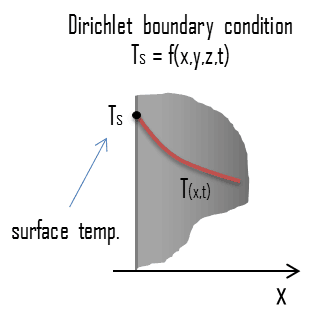
\includegraphics[height=4.8cm, width=3.8cm]{dirichlet-temp.png}
           \end{tabular}
           & \begin{tabular}{l}
             \parbox{6cm}{%  change the parbox width as appropiate
            \begin{itemize}
            \item BVPs are extremely important as they are vital in the study of many multidisciplinary applications such as:
                \begin{itemize}
                    \item fluid mechanics
                    \item solid mechanics to heat transfer
                    \item electromagnetic potential
                \end{itemize}
            \end{itemize}
    }
        \end{tabular}  \\
    \end{tabular}
\end{frame}

\begin{frame}
\frametitle{What is the BVP?}
\begin{itemize}
    \item A BVP consists of a system of differential equations where a set of conditions is known, and whose solutions are to be found in a specified domain.
    \item It is opposed to the initial value problem, in which only the conditions on one extreme of the interval are known.
    \item Thus, the choice of the boundary condition is fundamental for the resolution of the given system since it will determine its accuracy, and in some cases, its convergence.
\end{itemize}
\end{frame}

 \begin{frame}  
    \frametitle{What is the BVP?}
    \begin{tabular}{cl}  
        \begin{tabular}{cr}
           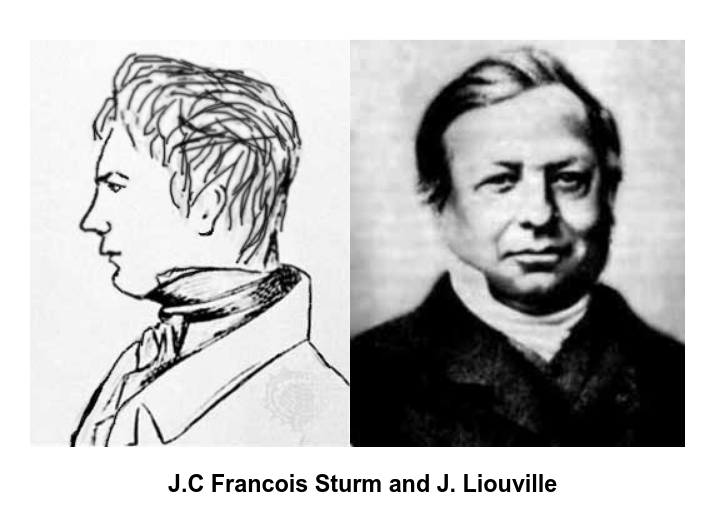
\includegraphics[height=4cm, width=4cm]{JCL.png}
           \end{tabular}
           & \begin{tabular}{l}
             \parbox{6cm}{%  change the parbox width as appropiate
            J.C Francois Sturm and J. Liouville studied the conditions which guarantee the existence and uniqueness of BVP solutions and how boundary conditions influence them, specially on well-posed systems.
    }
        \end{tabular}  \\
    \end{tabular}
     \begin{center} \textit{In this work, we study the Dirichlet BVP problem for given conditions along the boundary of the domain in the x-y plane.} \end{center}
\end{frame}

\begin{frame}  
    \frametitle{What is the BVP?}
    \begin{tabular}{cl}  
           \begin{tabular}{c}
           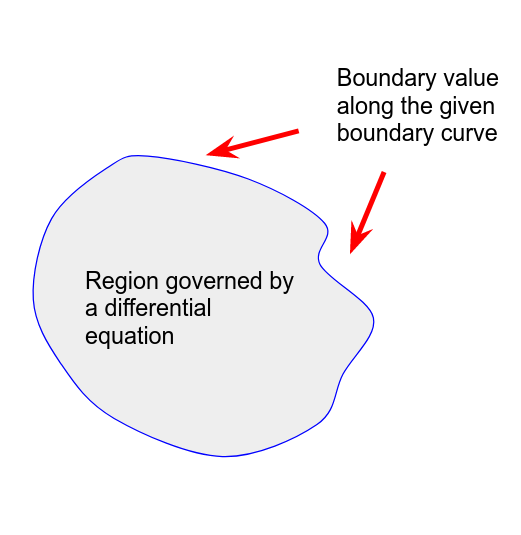
\includegraphics[height=4.8cm, width=3.8cm]{BVP.png}
           \end{tabular}
           & \begin{tabular}{l}
             \parbox{6cm}{%  change the parbox width as appropiate
            \begin{itemize}
            \item The Dirichlet problem was initially intended to particularly find solutions to the Laplace's equation.
            \item Its main purpose is to find the solution of a second-order elliptic equation which is regular in the domain.
            \item Note: the Dirichlet problem for harmonic functions always has a solution, and that solution is unique, when the boundary is sufficiently smooth and \textit{f(s)} is continuous. 
            \end{itemize}
    }
        \end{tabular}  \\
    \end{tabular}

\end{frame}

\begin{frame}
\frametitle{Objectives}
\begin{itemize}
    \item Discuss the general formulation of the Dirichlet problem and its applicability to specific problems.
    \item Develop a set of Octave scripts to solve two given Dirichlet BVPs.
    \item Apply the shooting and Newton's numerical methods to approximate the solutions of the given systems.
\end{itemize}
\end{frame}
%----------------------------------------------------------
% Dirichlet BVP Formulation (Jomarie)
%----------------------------------------------------------
% Done
\begin{frame}
\frametitle{Dirichlet Boundary Value Problem Formulation} % part 1
The general Dirichlet-type BVP for a function $y(t)$ in an interval [a,b] is given by:
\begin{equation}\label{1}
    \begin{cases}
        y''(t)=f(t,y(t),y'(t)), \ \ \ \ \ a < t < b,\\
        y(a)=\alpha, \ \ \ \ \ y(b)=\beta,
    \end{cases}
\end{equation}
where $\alpha, \beta$ are given numbers.This linear two-point BVP can be solved by forming a combination of the solutions to two initial value problems, the so called shooting method.
\end{frame}
%----------------------------------------------------------
% Done
\begin{frame}
\frametitle{Dirichlet Boundary Value Problem Formulation} % part 2
Let $y(t,\gamma)$ be the solution of the initial value problem:
\begin{equation}\label{2}
        \begin{cases}
            y''(t)=f(t,y(t),y'(t)),  \ \ \ \ \ a < t < b,\\
            y(a)=\alpha,  \ \ \ \ \ y'(a)=\gamma
        \end{cases}
    \end{equation}
We can now find a value for $\gamma$ such that $y(b,\gamma)=\beta$. Thereby, we can find a root $\gamma*$ for the equation $y(b,\gamma)-\beta=0$.
\end{frame}
%----------------------------------------------------------
% Done
\begin{frame}
\frametitle{Dirichlet Boundary Value Problem Formulation} % part 3
If we define 
\begin{equation}\label{3}
        g(\gamma) \equiv y(b,\gamma) - \beta
\end{equation}

we can find a root $\gamma*$ of function $g$ with Newton's Method. Each evaluation of function $g$ requires finding the solution of initial value problem (\ref{2}). Also, $g'(\gamma)$ must be found in order to use Newton's Method. Taking the derivative in (\ref{3}), we have that $g'(\gamma) = u(b)$, where:
$$
u(t)=\frac{\partial y}{\partial \gamma}(t,\gamma)
$$
(We are omitting the dependency of $u$ in $\gamma$ for simplification purposes).
\end{frame}

%----------------------------------------------------------
% Done
\begin{frame}
\frametitle{Dirichlet Boundary Value Problem Formulation} % part 4
By finding the derivative of the initial value problem (\ref{2}) with respect to $\gamma$, it can be concluded that $u(t)$ is the solution of the following initial value problem:

    \begin{equation}\label{4}
        \begin{aligned}
            \begin{cases}
                u''(t)=\frac{\partial f}{\partial y}(t,y(t,\gamma),y'(t,\gamma))u(t)+\frac{\partial f}{\partial z}(t,y(t,\gamma),y'(t,\gamma))u'(t),\\
                u(a)=0, \ \ \ \ \ u'(a)=1, \ \ \ a < t < b.
            \end{cases}
        \end{aligned}
    \end{equation}

Given the function $y(t,\gamma)$, this is a linear problem for $u(t)$; thus the initial value problems (\ref{2}) and (\ref{4}) can be numerically solved in parallel.
\end{frame}

%----------------------------------------------------------
% Done
\begin{frame}
\frametitle{Selected Boundary Value Problems Formulation} %Jomarie
Consider the first problem defined by:  
\begin{equation}\label{5}
    \begin{cases}
        y''(t)=\frac{1}{8}(32+2t^3-y(t)y'(t)), \ \ \ \ \  1<t<3, \\
        y(1)=17, \ \ \ \ \ y(3)=\frac{43}{3}.
    \end{cases}
\end{equation} 

Let $y(t,\gamma)$ be the solution of the initial value problem

\begin{equation}\label{6}
    \begin{cases}
      y''(t)=\frac{1}{8}(32+2t^3-y(t)y'(t)), \ \ \ \ \ 1<t<3,\\
        y(1)=17, \ \ \ \ \ y'(1)=\gamma,\\
    \end{cases}
\end{equation}
\end{frame}

%----------------------------------------------------------
% Done
\begin{frame}
\frametitle{Selected Boundary Value Problems Formulation} % (Jomarie)
Let $u(t)=\frac{\partial y}{\partial \gamma}(t, \gamma)$ be the solution of the following initial value problem:
    \begin{equation}\label{7}
        \begin{cases}
            u''(t)=-\frac{1}{8}y'(t)u(t) -\frac{1}{8}y(t)u'(t),\ \ \ \ 1 < t < 3, \\
            u(0)=0, \ \ \ \ \ u'(0)=1.
        \end{cases}
    \end{equation}
    
Thus we proceed to calculate the root of the following equation:
\begin{equation}\label{8}
g(\gamma)\equiv y(1,\gamma)-\frac{43}{3}=0.
\end{equation}
\end{frame}
%----------------------------------------------------------
% Done
\begin{frame}
\frametitle{Selected Boundary Value Problems Formulation} % (Jomarie)
Using the substitutions $u_1(t)=y(t)$, $u_2(t)=y'(t)$, $u_3(t)=u(t)$ and $u_4(t)=u'(t)$ we can transform (\ref{6}) to a first-order system:
\begin{equation}\label{9}
    \begin{cases}
        u'_1(t)=u_2(t)\\
        u'_2(t)=\frac{1}{8}(32+2t^3-u_1(t)u_2(t))\\
        u'_3(t)=u_4(t)\\
        u'_4(t)=-\frac{1}{8}u_2(t)u_3(t) -\frac{1}{8}u_1(t)u_4(t),
    \end{cases}
\end{equation}
where $u_1(1)=17$, $u_2(1)=\gamma$, $u_3(1)=0$, and $u_4(1)=1$.
By solving this system, we find the value of $g(\gamma)$. Now that we know the values of $g(\gamma)$ and $g'(\gamma)$, which is u(3), we proceed to calculate $\gamma*$ with Newton's Method.
\end{frame}

%----------------------------------------------------------
% Done
\begin{frame}
\frametitle{Selected Boundary Value Problems Formulation} % (Jomarie)
Consider the second problem defined by:

\begin{equation}\label{10}
    \begin{cases}
        y''(t)=\frac{1+(y'(t))^2}{1+y(t)}, \ \ \ \ \  0<t<5, \\
        y(0)=1, \ \ \ \ \ y(5)=10.
    \end{cases}
\end{equation} 

Let $y(t,\gamma)$ be the solution of the initial value problem

\begin{equation}\label{11}
    \begin{cases}
      y''(t)=\frac{1+(y'(t))^2}{1+y(t)}, \ \ \ \ \  0<t<5, \\
        y(0)=1, \ \ \ \ \ y'(0)=\gamma .\\
    \end{cases}
\end{equation}
    
\end{frame}

%slide 12
\begin{frame}
\frametitle{Selected Boundary Value Problems Formulation} % (Jomarie)
Let $u(t)=\frac{\partial y}{\partial \gamma}(t, \gamma)$ be the solution of the following initial value problem:
    \begin{equation}\label{12}
        \begin{cases}
            u''(t)=-\frac{1+(y'(t))^2}{(1+y(t))^2}u(t)+\frac{2y'(t)}{1+y(t)}u'(t),\ \ \ \ 0 < t < 5, \\
            u(0)=0, \ \ \ \ \ u'(0)=1.
        \end{cases}
    \end{equation}
    
Thus we proceed to calculate the root of the following equation:
\begin{equation}\label{13}
g(\gamma)\equiv y(0,\gamma)-10=0.
\end{equation}
\end{frame}

%slide 13
\begin{frame}
\frametitle{Selected Boundary Value Problems Formulation} %(Jomarie)
Using the substitutions $u_1(t)=y(t)$, $u_2(t)=y'(t)$, $u_3(t)=u(t)$ and $u_4(t)=u'(t)$ we can transform (\ref{11}) to a first-order system:

\begin{equation}\label{14}
    \begin{cases}
        u'_1(t)=u_2(t)\\
        u'_2(t)=\frac{1+(u_2(t))^2}{1+u_1(t)}\\
        u'_3(t)=u_4(t)\\
        u'_4(t)=-\frac{1+(u_2(t))^2}{(1+u_1(t))^2}u_3(t)+\frac{2u_2(t)}{1+u_1(t)}u_4(t),
    \end{cases}
\end{equation}
where $u_1(0)=1$, $u_2(0)=\gamma$, $u_3(0)=0$, and $u_4(0)=1$. By solving this system, we find the value of $g(\gamma)$. Now that we know the values of $g(\gamma)$ and $g'(\gamma)$, which is u(5), we proceed to calculate $\gamma*$ with Newton's Method.
    
\end{frame}

\begin{frame}
\frametitle{Numerical Methods: Shooting Method}
\begin{itemize}
    \item The shooting method was selected to find the solutions of the given BVPs. This method transforms the BVP into a combination of two initial value problems and proceeds to calculate the root of the equation given by (\ref{3}).
    \item In the previous section, the original systems were transformed into first-order systems to find their numerical solutions, particularly to find the value of $g(\gamma)$.
    \begin{center}
    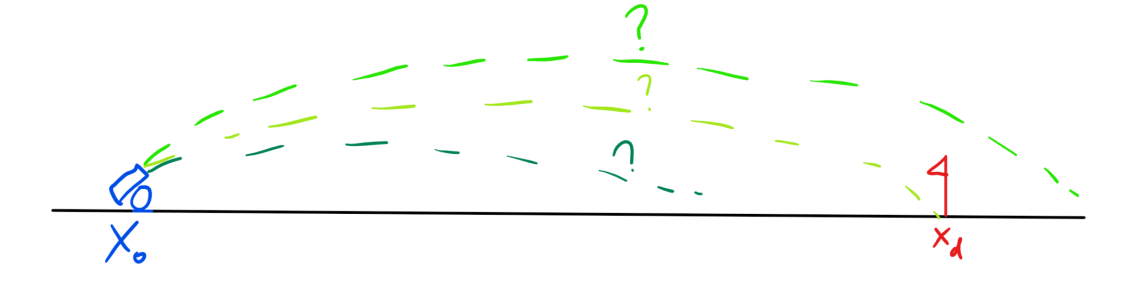
\includegraphics[height=3cm, width=8cm]{ShootingMethodSkech.png}
    \end{center}
\end{itemize}
\end{frame}

\begin{frame}
\frametitle{Numerical Methods: Newton Method}
\begin{itemize}
    \item These solutions were found using an ODE45 solver, which implements a combination of order four and order five Runge-Kutta methods to evaluate given differential equations systems.
    \item Once the systems were solved and the solution of $g(\gamma)$ was found, the Newton method was applied to approximate a numerical root of $\gamma$*.
    \item This method was selected over the bisection and secant methods due to its superior order of convergence and computational speed. The availability of a continuous derivative of $f$ reaffirmed this selection.
\end{itemize}
\end{frame}

 \begin{frame}
\frametitle{Numerical Methods: Newton Method}
    Newton's method supposes that the given function $f$, which in this problem is represented by $g(\gamma)$, is differentiable. Then, the tangent line to $f$ in the point $(x_0, f(x_0))$ is given by the equation
    
        \begin{equation}\label{15}
            y = f(x_0) + f'(x_0)(x-x_0) 
        \end{equation}
    which is also the first degree Taylor polynomial. Therefore, an approximation of $f$ can be found using this tangent line and defining $x_1$ as the x-intercept of the line. That is:

    \begin{equation}\label{16}
        x_1 = x_0 - \frac{f(x_0)}{f'(x_0)}, \ \ \ \ \ f'(x_0) \neq 0. 
    \end{equation}
\end{frame}

 \begin{frame}
\frametitle{Numerical Methods: Newton Method}
    Thus, this process can be repeated as long as it is needed, obtaining the following recursion:
    
        \begin{equation}\label{17}
            \begin{cases}
                x_{n+1} = x+n - \frac{f(x_n)}{f'(x_n)} \ \ \ \ \ n \geq 0,  \\
                x_0 \ \ given, \\
            \end{cases}
        \end{equation}
    
    which is generally described as a fixed point iteration. Newton's method convergence is covered by \textit{Theorem 1} (next slide). 
\end{frame}

 \begin{frame}
\frametitle{Numerical Methods: Newton Method}
    In order to analyze the order of convergence of the Newton method we need to define the following theorems: \newline \newline
    \noindent \textbf{Theorem 1}. Suppose that $f : \mathbb{R} \rightarrow \mathbb{R}$ is a function $C^2$ in a neighborhood of the scalar $\alpha$, where $f(\alpha) = 0, f'(\alpha) \neq 0.$ Then, if $x_0$ is selected close enough to $\alpha$, the interations from (\ref{17}) converge to $\alpha$. Furthermore,

    \begin{equation}\label{18}
        \lim_{n\to\infty} \frac{\alpha - x_{n+1}}{(\alpha - x_n)^2} = - \frac{f''(\alpha)}{2f'(\alpha)}
    \end{equation}
    \noindent that is, $(x_n)$ converges to $\alpha$ with convergence order of $p = 2$. The proof of this theorem is discussed in detail on professor's P. Negr\'{o}n book. 
\end{frame}

 \begin{frame}
\frametitle{Numerical Methods: Newton Method}
    \noindent \textbf{Theorem 2}. Suppose $f \in C^{n+1}(\alpha, \beta)$ and $a \in (\alpha,\beta)$. Let $R_n (x) = f(x) - p_n(x)$ the error of approximating $f$ with $p_n$. Then:
    \begin{ssmall}
        \begin{equation}\label{19}
            R_n(x) = \frac{1}{n!} \int_{a}^{x} f^(n+1)(\xi)(x-\xi)^n d\xi = \frac{f^(n+1)(c_x)}{(n+1)!}(x-a)^{n+1}, x \in (\alpha, \beta),
        \end{equation}
    \end{ssmall}
    \noindent where $c_x$ is a number between $a$ and $x$. \newline 
    
    Therefore, using the Taylor Theorem (\textit{Theorem 2}) we can write:

    \begin{equation}\label{20}
        f(\alpha) = f(x_n) + f'(x_n)(\alpha - x_n) + \frac{1}{2} f''(\xi_n)(\alpha - x_n)^2 \ ,
    \end{equation}
    where $\xi_n$ is between $\alpha$ and $x_n$. Since $f'(\alpha) \neq 0$ and $f'$ is continuous, there exists a closed interval $I$ around $x=\alpha$ such that $f'(\alpha) \neq 0$ for $x \in I$. 
\end{frame}

 \begin{frame}
\frametitle{Numerical Methods: Newton Method}
    Therefore we can define the number $M$ as
    
        \begin{equation}\label{21}
            M = \frac{1}{2} \frac{max_{x \in I}|f''(x)|}{min_{x \in I}(f'(x))}
        \end{equation}
    
    which is finite and exists. Note that the selection of the initial value $x_0$ is extremely important to guarantee convergence. \newline
    
    From \textit{Theorem 1} and (\ref{21}), it can be observed that if $M|\alpha - x_0| < 1$, then the iterations of this method converge to the root. Unfortunately, this estimate is not practical since $M$, which is given by (\ref{21}), is in general hard or impossible to calculate.
    % Decir en la presentacion que:  every estimate or known detail from the system is vital to improve the convergence possibilities of this method. Techniques such as plotting $f$ or using the bisection method to understand the region more precisely, could be used to approximate this value correctly and ensure convergence. 

\end{frame}

 \begin{frame}
\frametitle{Numerical Methods: Newton Method}
    Lastly, a heuristic criterion to stop the iterations of this method, supposing iterations ($x_n$) are close to the root $\alpha$, could be given by:
    
        \begin{equation}\label{22}
            Rel(x_n) = \frac{\alpha - x_n}{\alpha} \approx \frac{x_{n+1} - x_n}{x_n}.
        \end{equation}
    
    Thus, if $|x_{n+1} - x_n| \leq |x_n|10^{-t}$ there are approximately $t$ significant numbers in $x_n$ as an approximation of $\alpha$. \newline
    
    The main possible sources of errors of this work reside on the ODE solvers and the Newton method. The parameters of absolute tolerance and max step-size were set to $10^{-6}$ and $10^{-3}$ respectively. Similarly, the tolerance of the Newton method was set to $10^{-5}$, in order to control the accuracy of the calculated root value. 
\end{frame}

%slide 15
\begin{frame}
\frametitle{Computational Analysis} % part 1
\begin{itemize}
    \item Using the Octave interpreter, we programmed:
    \item[]
    \begin{itemize}
        \item Systems of equations
        \item[]
        \item Newton method algorithm
        \item[]
        \item $g$ function calculator
        \item[]
        \item Driver for finding the solutions of the given systems
    \end{itemize}
\end{itemize}
\end{frame}

\begin{frame}[fragile]
\frametitle{Computational Analysis: Newthon Method} % part 1
The function for the Newton method was provided by P. Negr\'{o}n.
\ssmall{
\begin{lstlisting}
    function [x,iter]=newton(f,x0,tol,itermax)
        if nargin<3
           tol=1.0e-4;
        end
        if nargin<4
           itermax=20;
        end
        x=x0;
        normx=0;
        normz=inf;
        iter=0;
        while (normz>tol*normx)&(iter<=itermax)
            [f0,fp0]=feval(f,x);
            z=-fp0\f0;
            normz=norm(z,2);
            normx=norm(x,2);
            x=x+z;
            iter=iter+1;
        end
\end{lstlisting}
}
\end{frame}

\begin{frame}[fragile]
\frametitle{Computational Analysis: $g$ function} 
Then, the $g$ function is calculated by:
\begin{lstlisting}
    function [g,gp]= gfunc(gam,a,b,alf,bet)
      y0=[alf,gam,0,1]';
      [t,u]=ode45(@sistyu,[a,b],y0);
      m=size(u,1);
      g=u(m,1)-bet;
      gp=u(m,3);
    end
\end{lstlisting}
This function returns an approximation of the $g(\gamma)$ and $g'(\gamma)$ values when given the boundaries of the interval, and the $\alpha$ and $\beta$ constants.
\end{frame}
%----------------------------------------------------------
% Computational Analysis - A lot of work to do
%----------------------------------------------------------
% Driver program for the first BVP
\begin{frame}[fragile]
%fragile hace falta para listing, no me pregunten porqué
\frametitle{Computational Analysis: First BVP} % part 2
Functions for the first BVP are given by:
\begin{lstlisting}
function w=sistyu(t,u)
  w=zeros(4,1);
  w(1)=u(2);
  w(2)=f(t,u(1),u(2));
  w(3)=u(4);
  w(4)=fy(t,u(1),u(2))*u(3) + fz(t,u(1),u(2))*u(4);
end 
function w=f(t,y,z)
  w=(32+2*t^3-y*z)/8;
end
function w=fy(t,y,z)
  w=-z/8;
end
function w=fz(t,y,z)
  w=-y/8;
end
\end{lstlisting}
\end{frame}

\begin{frame}[fragile] %fragile hace falta para listing
\frametitle{Computational Analysis: First BVP} 
The driver program for the first BVP is given by:
\begin{lstlisting}
a=1.0;
b=3.0;
alf=17.0;
bet=43/3;

x=1:.1:3;
yexacta=x.^2+16./x;
tm=newton(@(x)gfunc(x,a,b,alf,bet),a)
y0=[alf,tm, 0,1]';
[t,u]= ode45(@sistyu, [a,b],y0);

plot(t,u(:,1),'k',x,yexacta,'k+')
xlabel('t'); ylabel('y');
legend('Numerical Solution', 'Exact Solution');
\end{lstlisting}
\end{frame}
%----------------------------------------------------------
% Driver program for the second BVP

\begin{frame}[fragile]
%fragile hace falta para listing, no me pregunten porqué
\frametitle{Computational Analysis: Second BVP} % part 2
Functions for the second BVP are given by:
\begin{lstlisting}
function w=sistyu(t,u)
  w=zeros(4,1);
  w(1)=u(2);
  w(2)=f(t,u(1),u(2));
  w(3)=u(4);
  w(4)=fy(t,u(1),u(2))*u(3) + fz(t,u(1),u(2))*u(4);
end 
function w=f(t,y,z)
  w=(1+z^2)/(1+y);
end
function w=fy(t,y,z)
  w=-(1+z^2)/((1+y)^2);
end
function w=fz(t,y,z)
  w= (2*z)/(1+y);
end
\end{lstlisting}
\end{frame}

\begin{frame}[fragile]
%fragile hace falta para listing, no me pregunten porqué
\frametitle{Computational Analysis: Second BVP} % part 2
The driver program for the second BVP is given by:
\begin{lstlisting}
a=0.0;
b=5.0;
alf=1.0;
bet=10.0;

tm=newton(@(x)gfunc(x,a,b,alf,bet),a)
y0=[alf,tm, 0,1]';
[t,u]= ode45(@sistyu, [a,b],y0);
plot(t,u(:,1))
xlabel('t'); ylabel('y')
\end{lstlisting}
\end{frame}
%----------------------------------------------------------
% Results - Done (Jomarie)
%----------------------------------------------------------
% Results - First BVP
\begin{frame}
\frametitle{Results: First BVP}
\begin{center}
\begin{figure}
    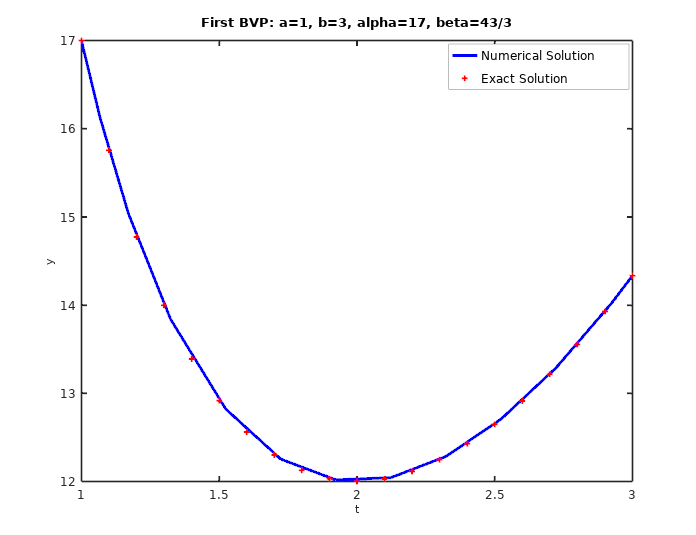
\includegraphics[scale=0.37]{ejemplo1b.png}
    \caption{\textit{Exact (red) and approximated solutions (blue) of the first BVP. The shooting method with initial parameters given by $a = 1.0, b = 3.0$, $\alpha = 17.0$, and $\beta = \frac{43}{3}$ was used for the approximation of the numerical solutions. The value of $\gamma*$ obtained was -14.000.}}
\end{figure}
\end{center}
\end{frame}

% Results - Second BVP
\begin{frame}
\frametitle{Results: Second BVP}
\begin{center}
\begin{figure}
    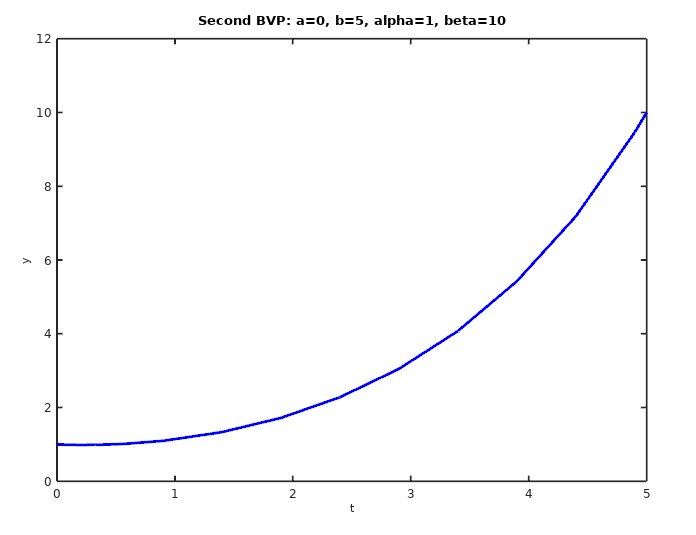
\includegraphics[scale=0.37]{ejercicio3b.png}
    \caption{\textit{Approximated solutions of the second BVP. The shooting method with initial parameters given by $a = 0.0, b = 5.0, \alpha = 1.0$, and $\beta = 10.0$ was used for the approximation of the numerical solutions. The value of $\gamma*$ obtained was -0.12175.}}
\end{figure}
\end{center}
\end{frame}
%----------------------------------------------------------
% Conclusions - Done
%----------------------------------------------------------
\begin{frame}
\frametitle{Conclusions}
\begin{itemize}
    \item The BVP has a wide range of multidisciplinary applications and can be approached using numerical methods.
    \item We have successfully developed a computational method for calculating the approximate solutions of two boundary value problems.
    \item It was proven that the proposed method could accurately find solutions for given systems when compared to exact solutions.
    \item The Newton method has proven to be fast and accurate when the continuous derivative of $f$ is present. Approximation errors can in fact be restricted with the parameters of absolute tolerance and max step size.
\end{itemize}
\end{frame}
%----------------------------------------------------------
% Future work - Done
%----------------------------------------------------------
\begin{frame}
\frametitle{Future Work}
\begin{itemize}
    \item Automation of the proposed set of scripts in order to calculate the derivatives using Matlab's symbolic libraries.
    \item[] 
    \item Further analysis of the Dirichlet problem using additional numerical methods such as the bisection and the secant algorithms to compare their accuracy against the Newton method.
    \item[] 
    \item Study the Neumann and Robin BVPs to validate the use of the proposed numerical methods.
\end{itemize}
\end{frame}

%----------------------------------------------------------
% References - Done
%----------------------------------------------------------
\begin{frame}
\frametitle{References}
 {\ssmall
 \begin{itemize}
    \item [1] Gustafson, Karl. \textit{Domain decomposition, operator trigonometry, Robin condition.} Contemporary Mathematics 218 (1998): 432-437.
    \item [2] P. Negr\'{o}n, \textit{Proyecto Computacional Final: Problema de Frontera}, UPR-Humacao, 2019. 
    \item [3] L\"{u}tzen, Jesper. \textit{Sturm and Liouville's work on ordinary linear differential equations. The emergence of Sturm-Liouville theory.} Archive for history of exact sciences 29.4 (1984): 309-376.
    \item [4] Rajurkar, R. K. \textit{General Solution of the Heat Equation, Wave Equation by Separation of Variables.}
    \item [5] A. Yanushauskas (2001) [1994], \textit{Dirichlet problem}, in Hazewinkel, Michiel (ed.), Encyclopedia of Mathematics, Springer Science+Business Media B.V. / Kluwer Academic Publishers, ISBN 978-1-55608-010-4
    \item [6] Adam, Badradeen, and Mohsin HA Hashim. \textit{Shooting method in solving Boundary Value Problem.} International Journal of Research and Reviews in Applied Sciences 21.1 (2014): 8.
    \item [7] P. Negr\'{o}n, \textit{Fundamentos del An\'{a}lisis Computacional.} University of Puerto Rico at Humacao (2015).
\end{itemize}
}
\end{frame}
%----------------------------------------------------------
% END DOCUMENT
%----------------------------------------------------------
\end{document}
%----------------------------------------------------------
% END DOCUMENT
%----------------------------------------------------------